\subsection{Feature Extraction}

\subsubsection{Datasets}
In this paper, we gather the charging stations logs from all the existing charging station companies who provide their services in Shanghai, with a total of over 2,000,000 lines. The log has a length of one month, from 2018/10 to 2018/11, in which an hourly summarize of each charging station is recorded, showing whether it's occupied or not.

\subsubsection{Hotspots}
From the data we gathered, we made several observations that benefits the features to be included in the model we present. We separate the data into different time frames in order to determine the overall difference among them, since charging network is a dynamic system.
\begin{figure}[!htbp]
	\begin{tabular}{cc}
		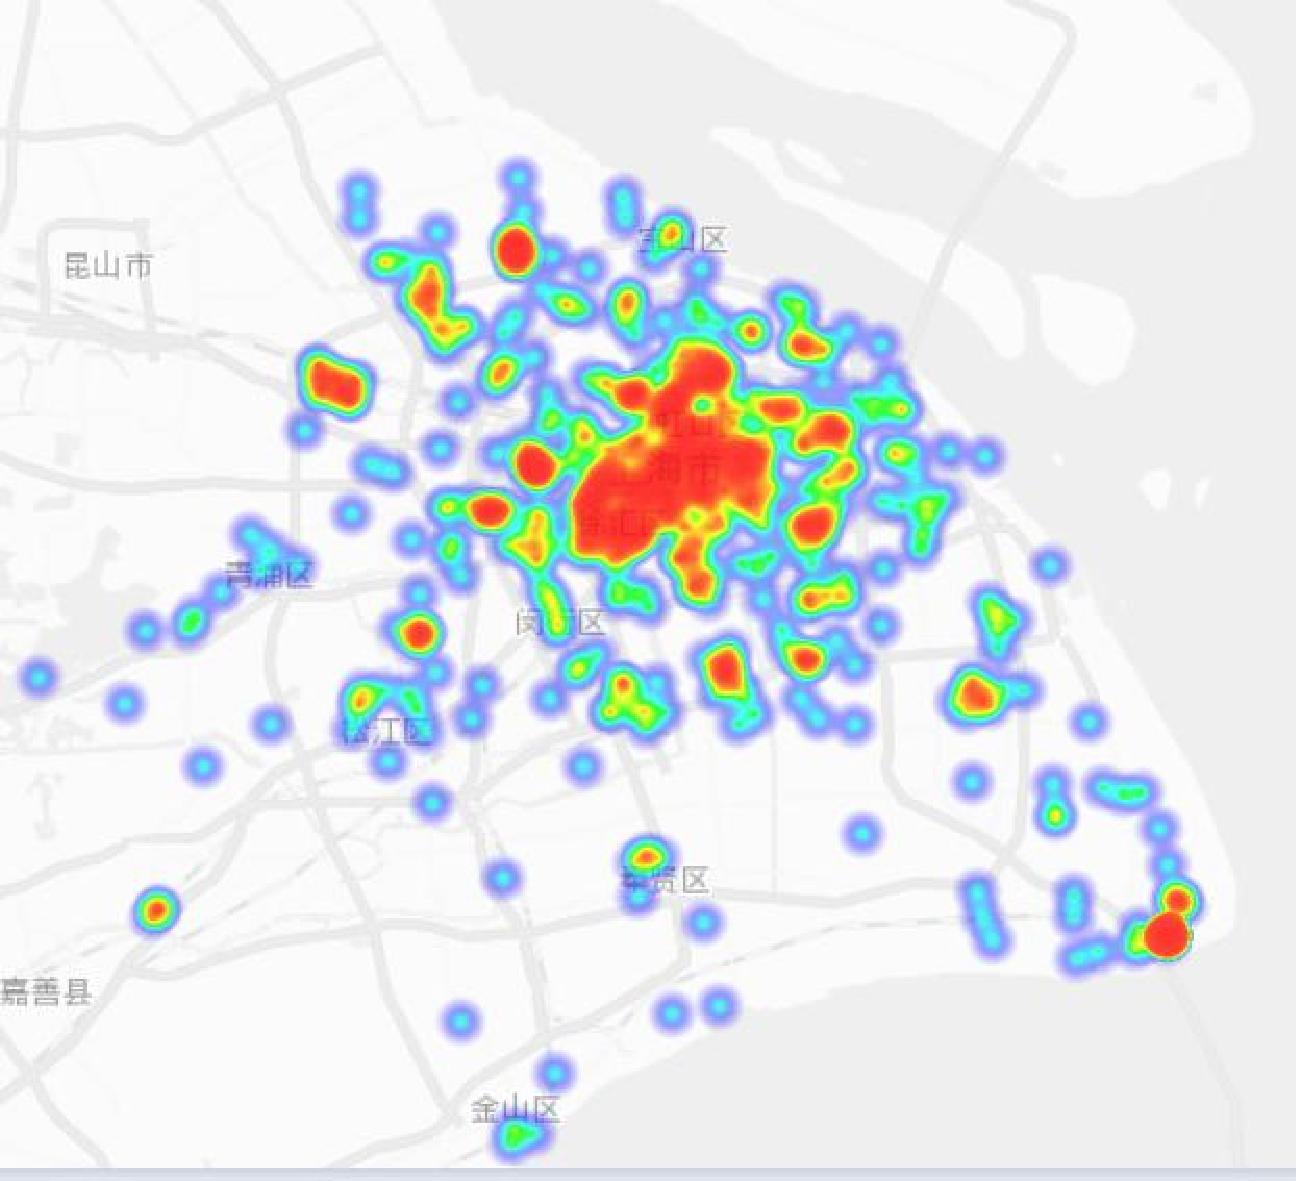
\includegraphics[width=0.45\columnwidth]{./figures/weekday.pdf} &  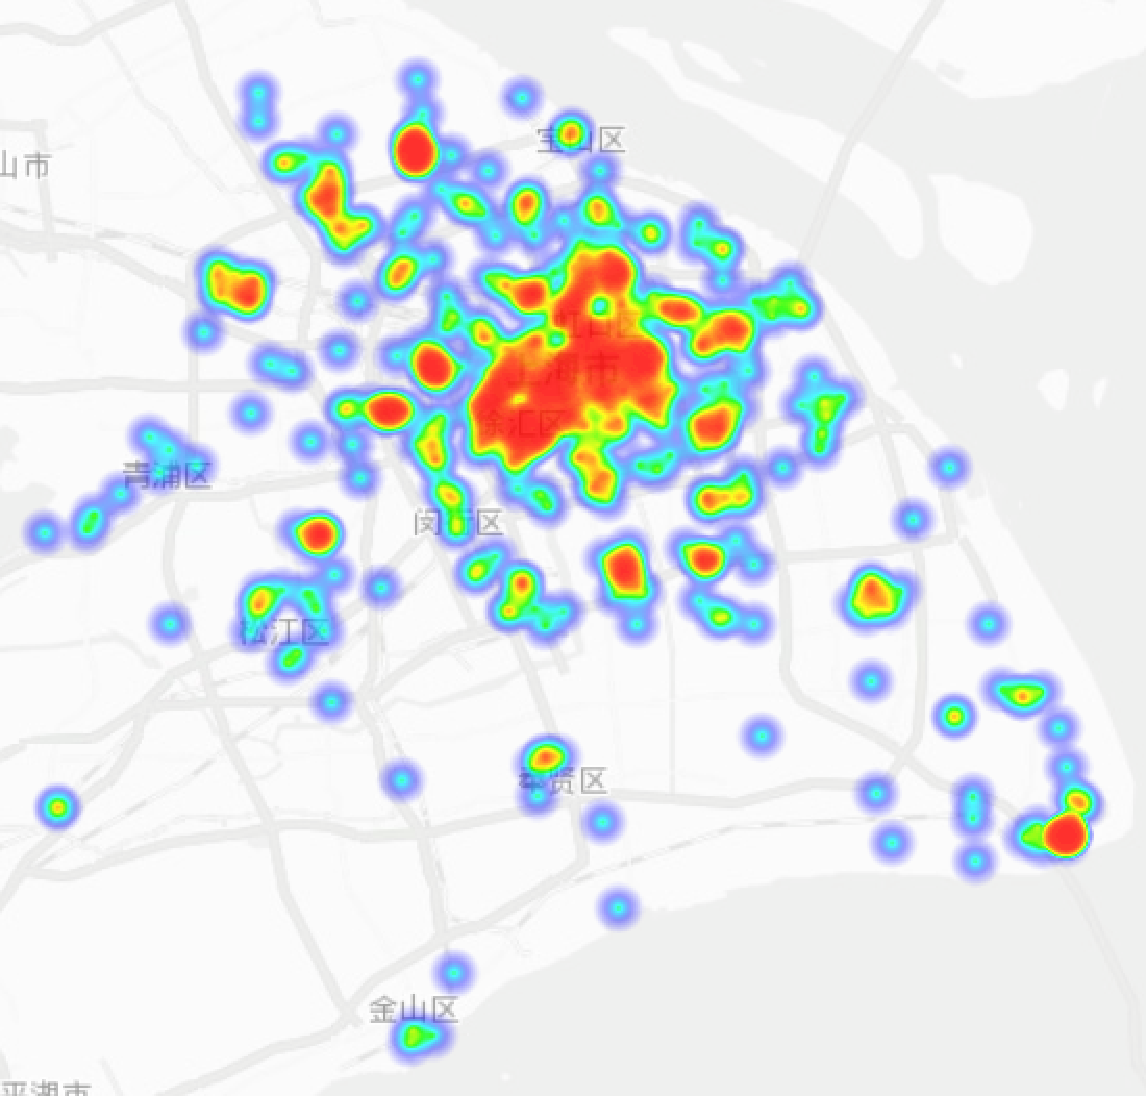
\includegraphics[width=0.45\columnwidth]{./figures/weekend.pdf} \\
		(a) Weekdays & (b) Weekends \\[6pt] 
		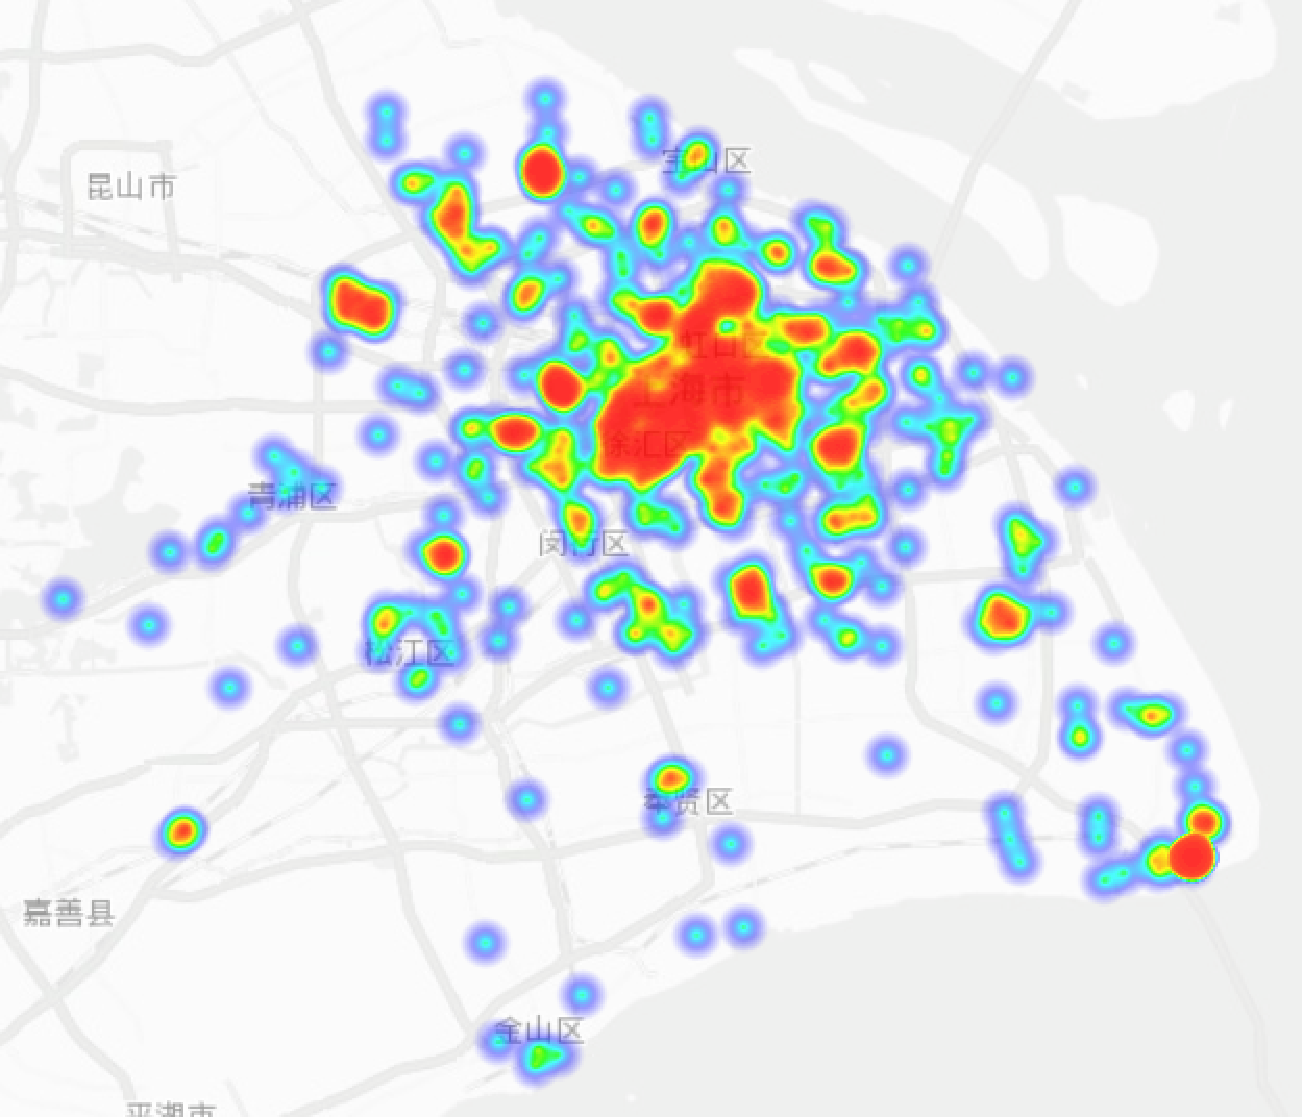
\includegraphics[width=0.45\columnwidth]{./figures/morning.pdf} &
		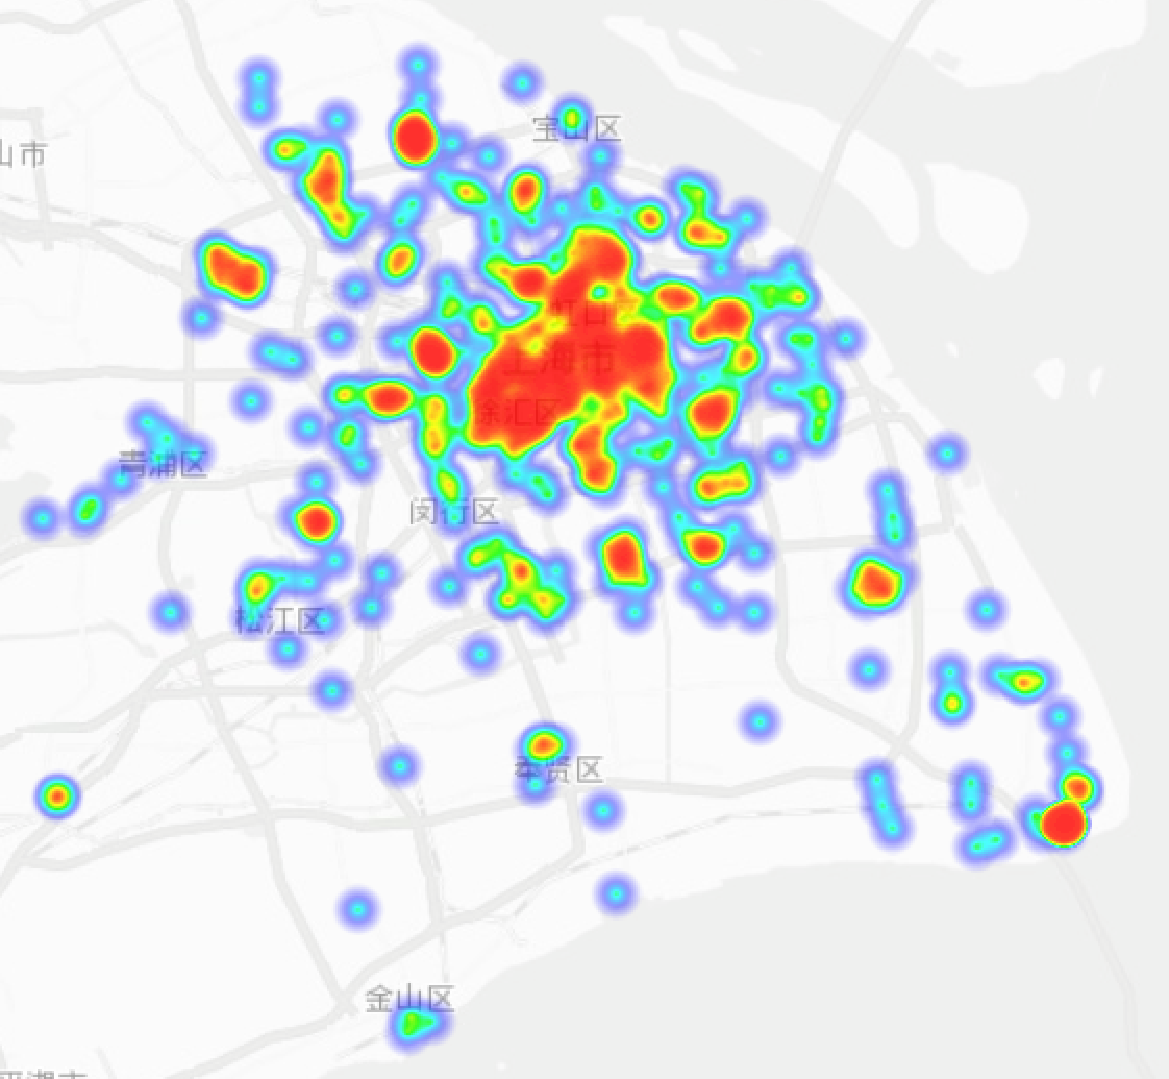
\includegraphics[width=0.45\columnwidth]{./figures/evening.pdf} \\
		(c) Mornings & (d) Evenings
	\end{tabular}
	\centering
	\caption{Charging Hotspots in Shanghai in Different Time Frames}
	\label{fig3}
\end{figure}
From Fig.\ref{fig3}, it is easy to notice that in different time frames, the charging hotspots stays at almost the same locations, meaning that during different time periods, the use rate of a given charging station is determined by its spatiotemporal context.


\subsubsection{Point Of Interest}
To the prosperity of Shanghai, there are so many points of interest(e.g., shopping malls, schools. estates, companies, etc.) located in the city.  Understanding the purpose of the trip by each person who participates in charging system will help us to analyze the use rate prediction. So, we need to extract the POI around each existing charging station. There are a lot of POIs in Shanghai. The POIs are very close to each other. We set a radius around each station and then collect the POIs within the radius. Based on our experiment, choosing a radius as 300 meters is proper. In our work, we get 80 different types of POI totally. Some of the POIs are very similar to each other. Therefore, we group 80 POIs in further step. By grouping POIs, we get 10 groups at last. Table.\ref{tab1} gives the groups and POIs in detail.

\begin{table}[!htbp]
	\caption{Groups of POIs}
	\begin{center}
		\begin{tabular}{|l|p{5cm}|}
			\hline
			Group & Points of interests\\
			\hline
			Food & chinese \& foreign restaurant, snack bar, cake \& dessert shop, cafe, bar\\
			\hline
			Hotels & star hotel, express hotel, apartment hotel\\
			\hline
			Shopping & shopping centers, department stores, supermarkets, convenience stores, home building materials, home appliances digital, shops, markets\\
			\hline
			Education & institutions of higher learning, middle schools, primary schools, kindergartens, adult education, parent-child education, special education schools, study agencies, research institutions, training institutions, libraries, science and technology museums\\
			\hline
			Cultural venue & press and publication, radio and television, art groups, art galleries, exhibition halls, cultural palaces\\
			\hline
			Medical & general hospitals, specialist hospitals, clinics, pharmacies, medical examination institutions, nursing homes, emergency centers, disease control centers\\
			\hline
			Car service & car sales, car repair, car beauty, auto parts, car rental, car inspection field\\
			\hline
			Transportation & airport, railway station, subway station, subway line, long-distance bus station, bus station, bus line, port, parking lot, refueling station, service area, toll station, bridge, charging station, roadside parking space\\
			\hline
			Estates & Office building, residential area, dormitory\\
			\hline
		\end{tabular}
		\label{tab1}
	\end{center}
\end{table}

\subsubsection{Distance}

In use rate prediction, we need to consider distance. People will not choose to park their electric cars for charging if the destination they planned to go is far away. In the system, a station with nearer distance to metro stations, financial centers and major functional buildings would easily be used more often. We select the nearest distance to the following to be the distance we considered as features: company, estate, hospital, metro station, shopping center and university. Fig.\ref{fig4} shows the total count of these important 'distance' POIs, from the figures we can see that these features almost satisfy the long tail distribution, which will be normalized in later work, see Preprocessing part.

\begin{figure}[!htbp]
	\begin{tabular}{cc}
		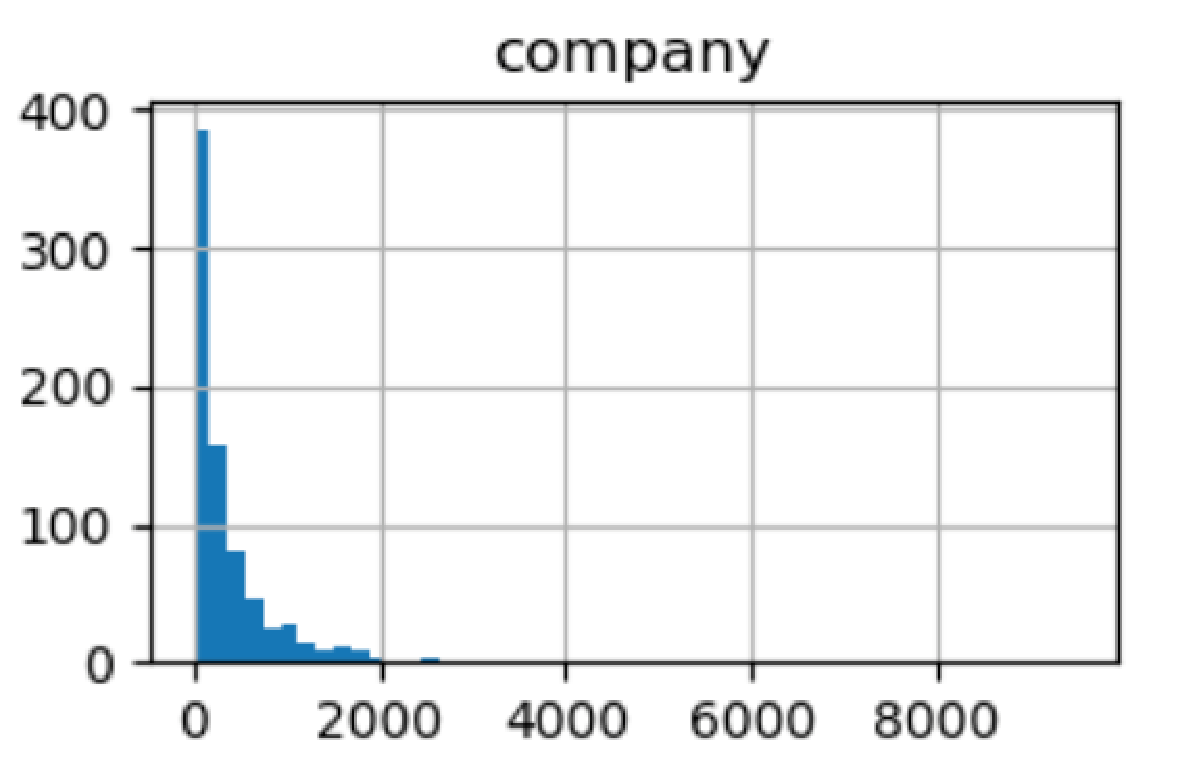
\includegraphics[width=0.45\columnwidth]{./figures/company.pdf} &  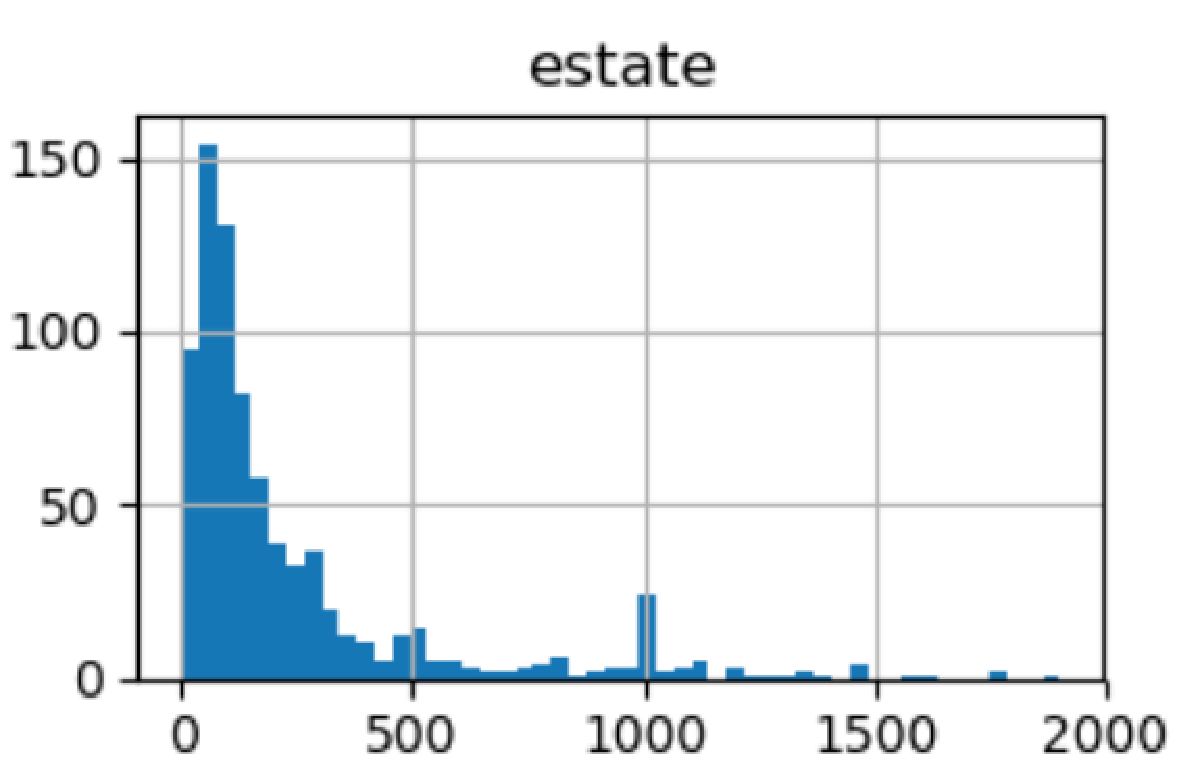
\includegraphics[width=0.45\columnwidth]{./figures/estate.pdf} \\
		(a) Company & (b) Estate \\[6pt] 
		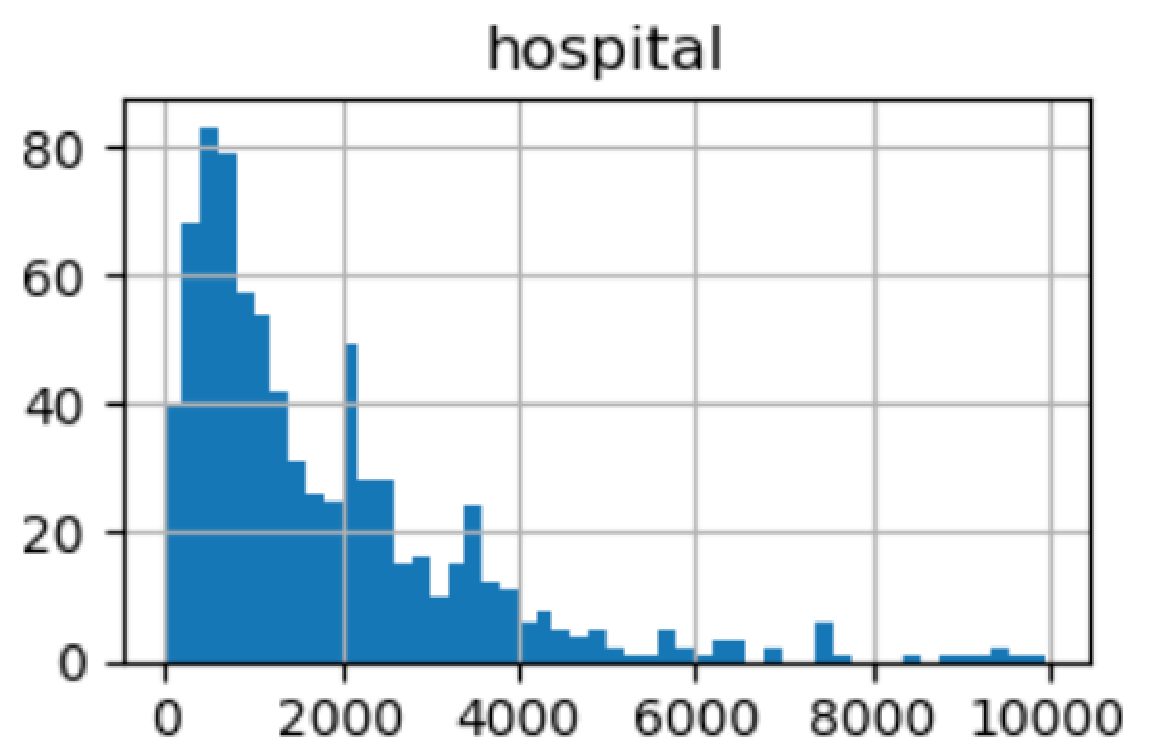
\includegraphics[width=0.45\columnwidth]{./figures/hospital.pdf} &
		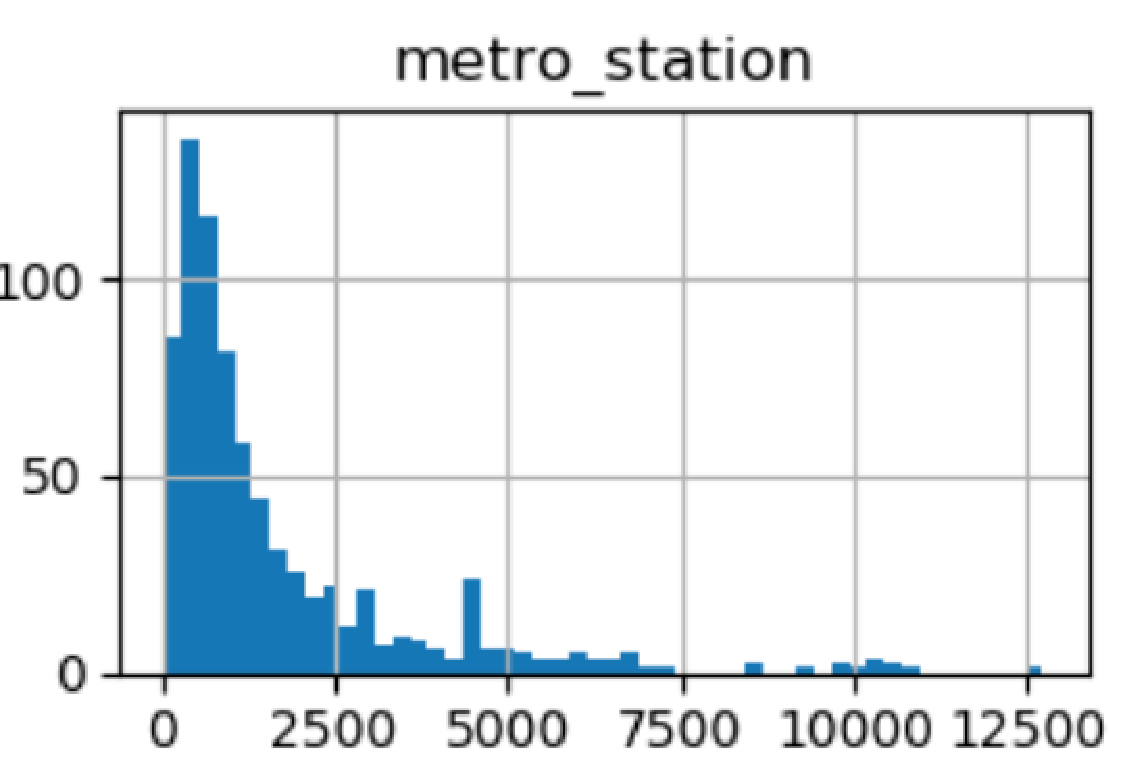
\includegraphics[width=0.45\columnwidth]{./figures/metro.pdf} \\
		(c) Hospital & (d) Metro Station \\
		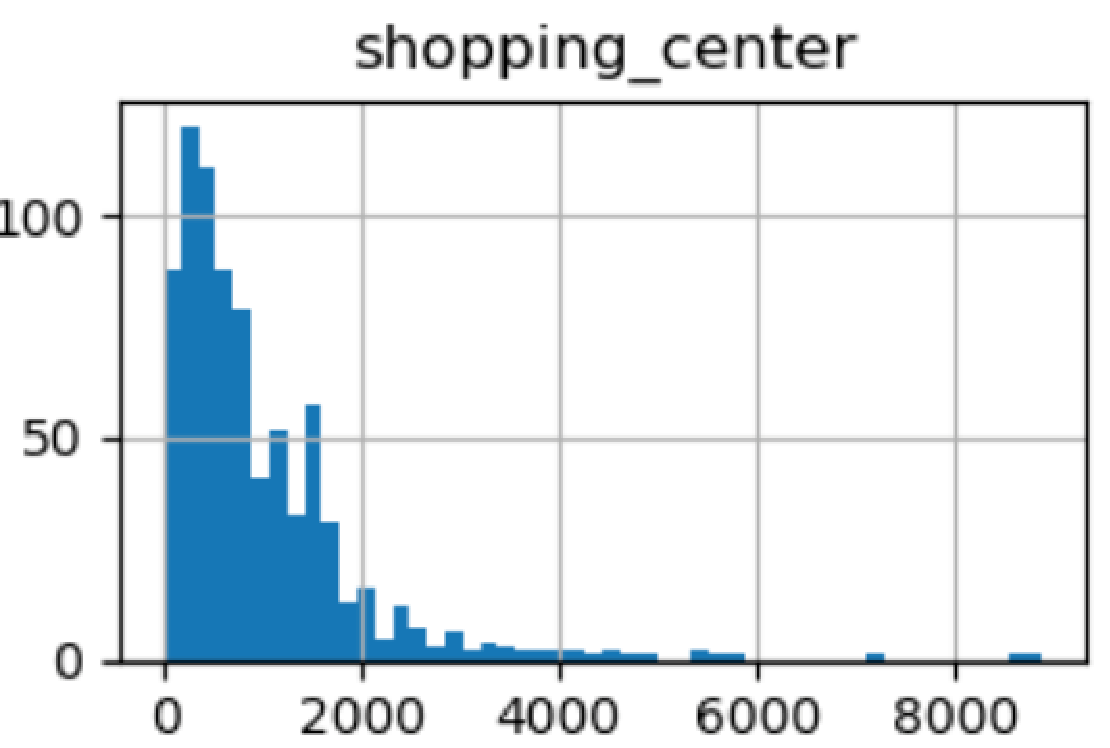
\includegraphics[width=0.45\columnwidth]{./figures/shop.pdf} 
		&
		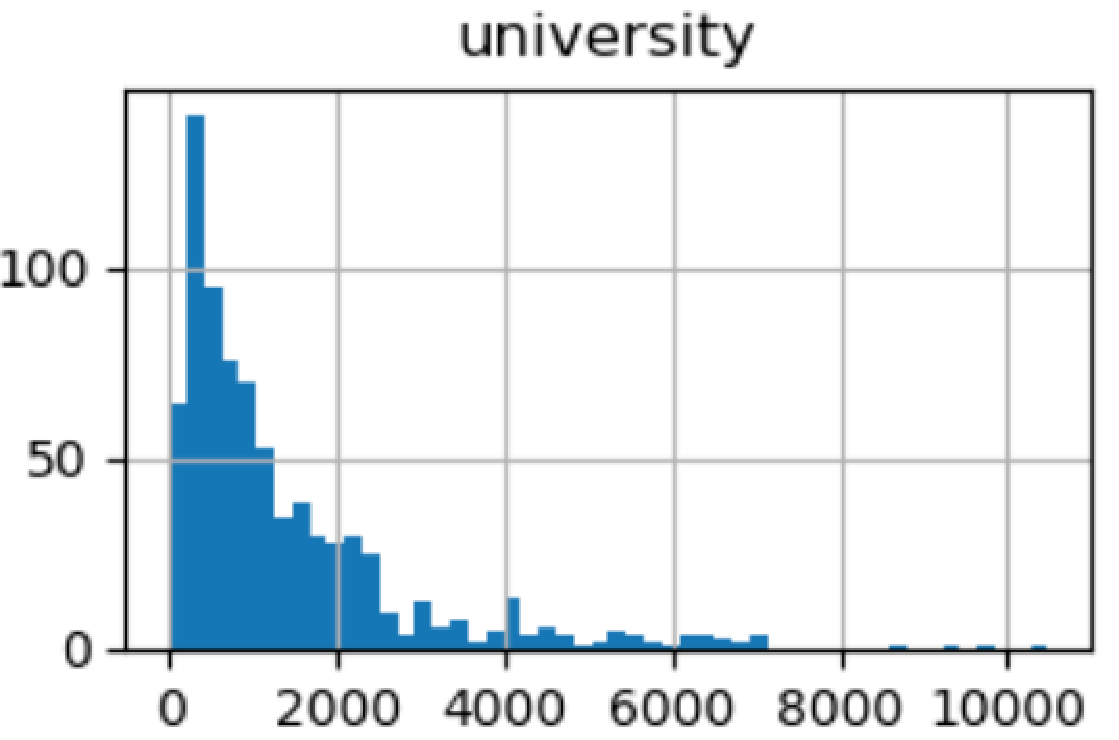
\includegraphics[width=0.45\columnwidth]{./figures/university.pdf} \\
		(e) Shopping Center & (f) University
	\end{tabular}
	\centering
	\caption{Count of Important POIs}
	\label{fig4}
\end{figure}

\subsubsection{Type \& Price}
By futher digging into the data, we find that there is a 0.3 correlation between price for charging and the use rate. Since there are two types of charging ports: DC and AC. We would include the number of ports and the price of both types in a charging station as one of its feature. Fig.\ref{fig5} shows the number of AC/DC type of stations's charging ports, as well as each type's charging cost fee. From the figures we observe that there are much more AC type charging ports than DC type ones, while the charging cost fee of them two are almost the same.

\begin{figure}[!htbp]
	\begin{tabular}{cc}
		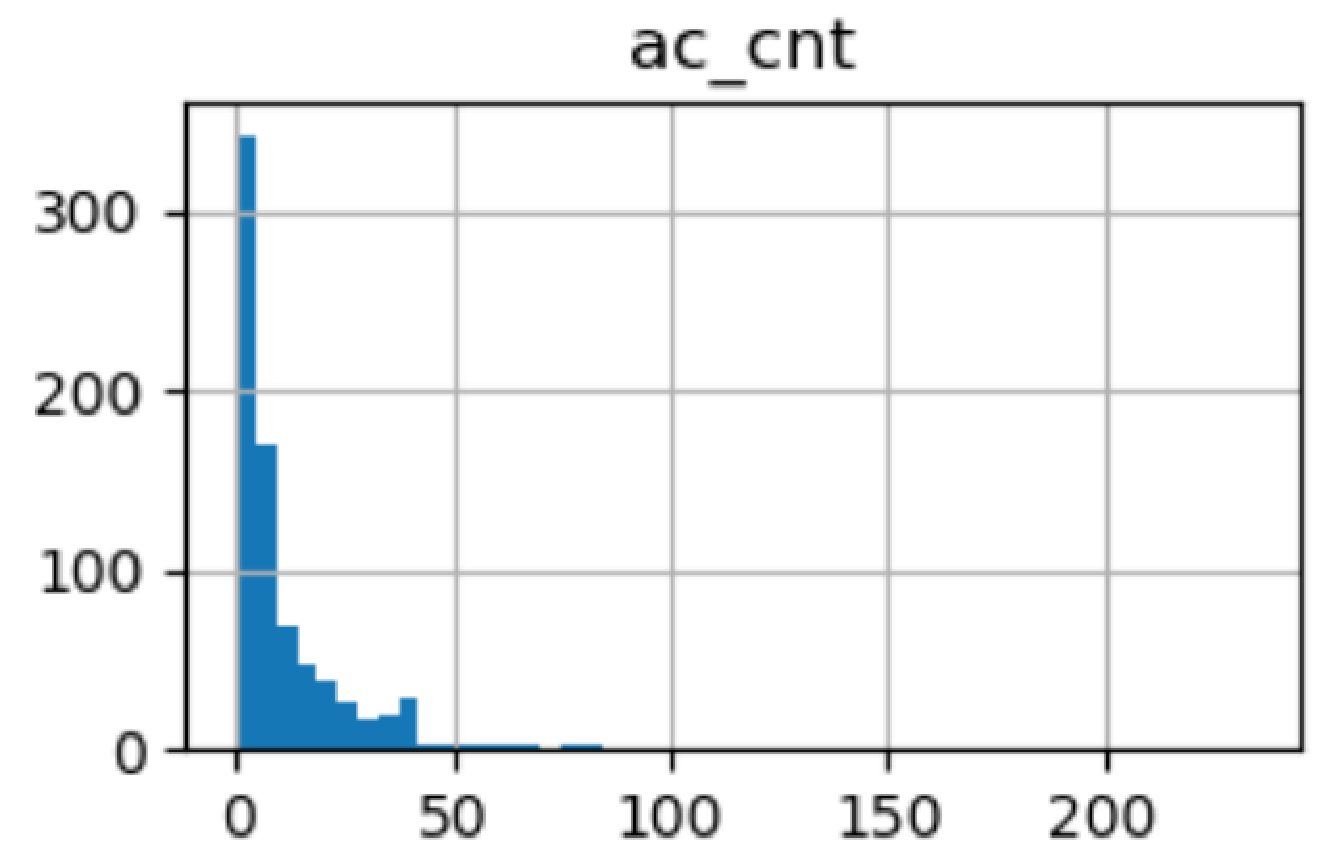
\includegraphics[width=0.45\columnwidth]{./figures/ac_cnt.pdf} &  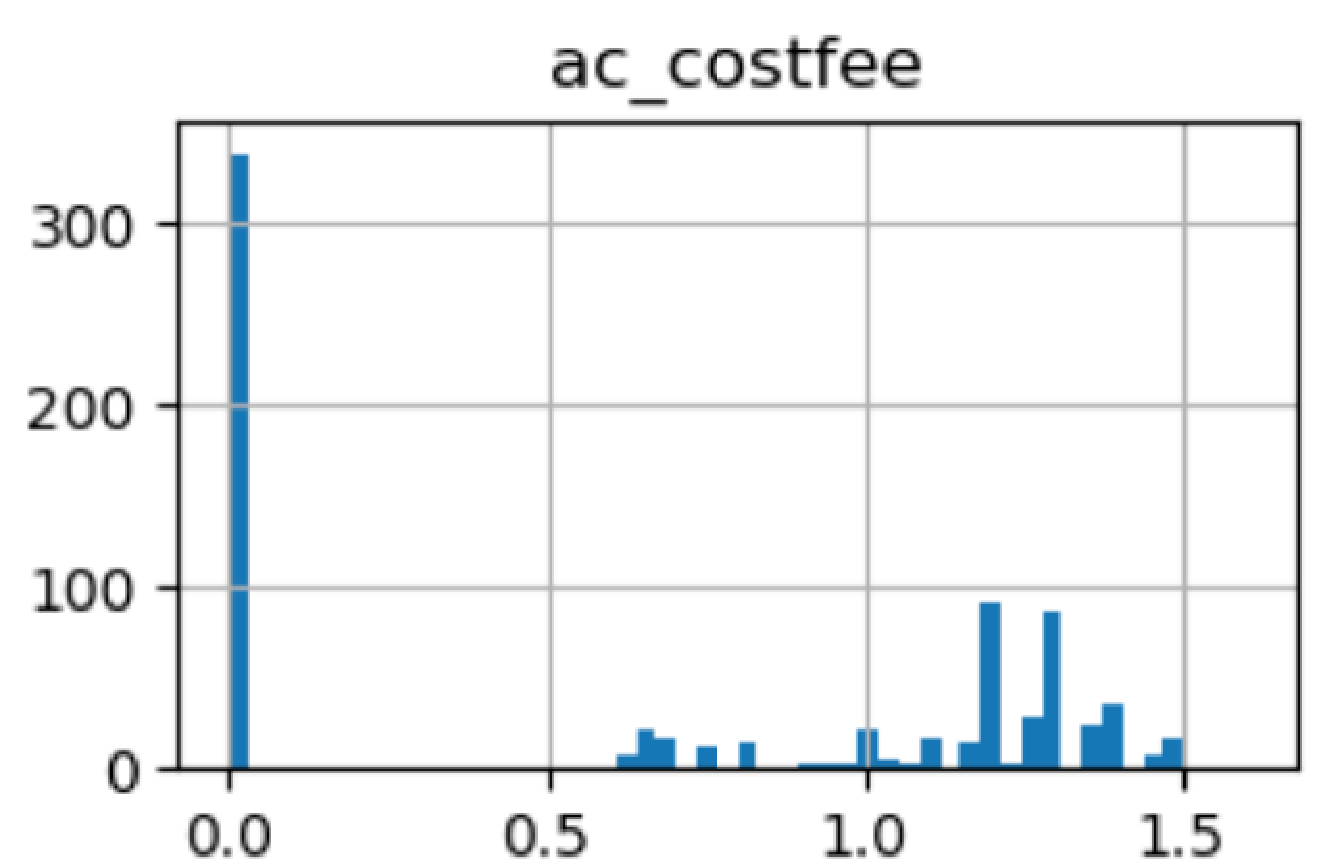
\includegraphics[width=0.45\columnwidth]{./figures/ac_fee.pdf} \\
		(a) AC\_Count & (b) AC\_Fee \\[6pt] 
		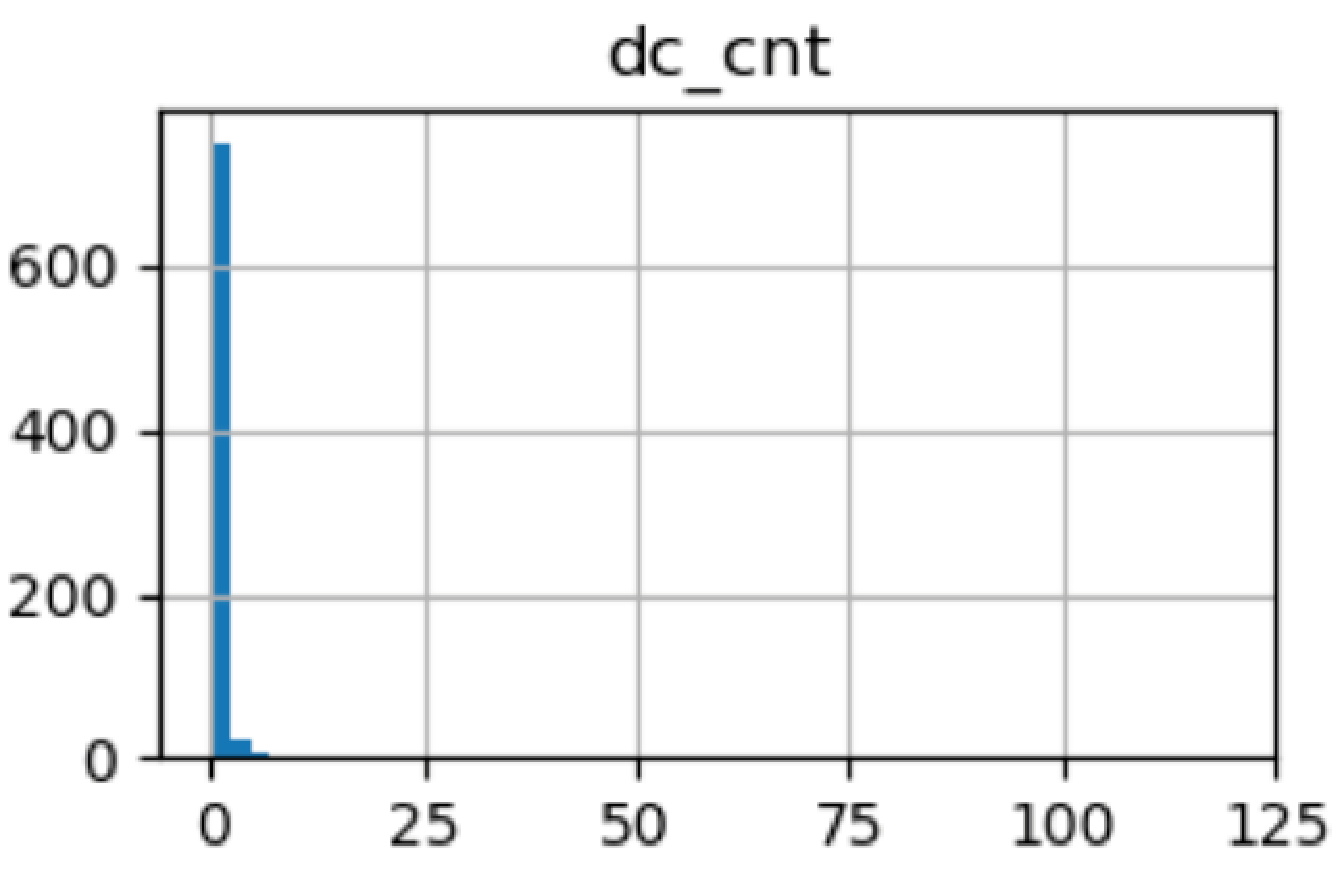
\includegraphics[width=0.45\columnwidth]{./figures/dc_cnt.pdf} &
		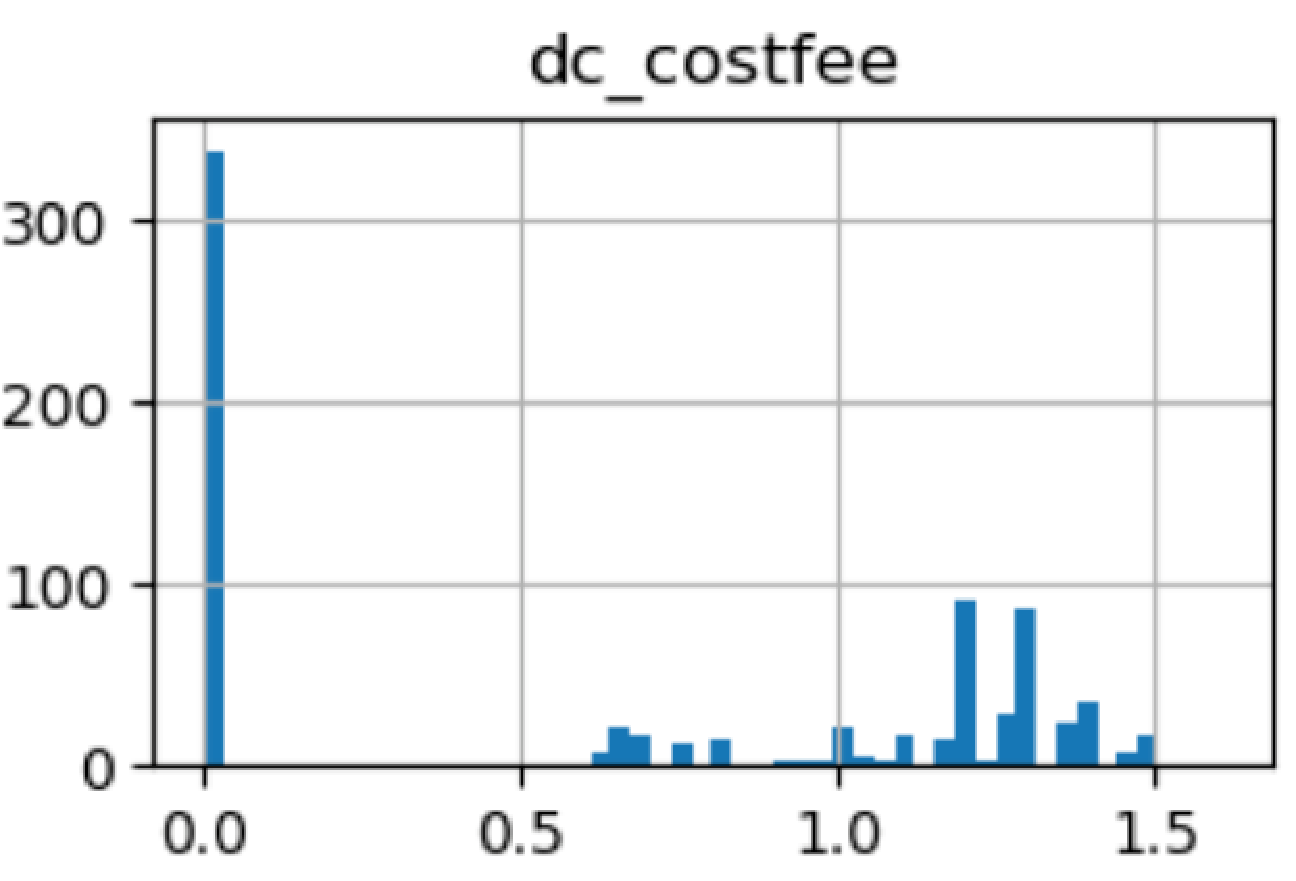
\includegraphics[width=0.45\columnwidth]{./figures/dc_fee.pdf} \\
		(c) DC\_Count & (d) DC\_Fee
	\end{tabular}
	\centering
	\caption{Charging Stations Types and Charging Cost Fee}
	\label{fig5}
\end{figure}

\subsubsection{Private or public}
By observing the data we've collected, it can be seen that most of the charging stations are private charging stations, which means they are typically used by electric buses and rent cars, or used by specific companies for their employees, accounting for over 70\% of the total charging stations. Also, since the private are used by more regular users(e.g., buses, companies employees), its use rate are 5\% higher compared to public ones. This alongside other observations will be taken into consideration.

\subsection{Spatio Temporal Data Based Framework}

\subsubsection{Ditricts}
There are 16 districts of station data in total, Fig.\ref{fig6} shows the distribution of charging stations in Shanghai. And for experiment , we separate them into two parts as urban area and suburb area. The final dataset for district prediction task contains the two parts of data, in urban part, 7 districts are included while in suburb part, 9 left districts are included.
\begin{figure}[!htp]
	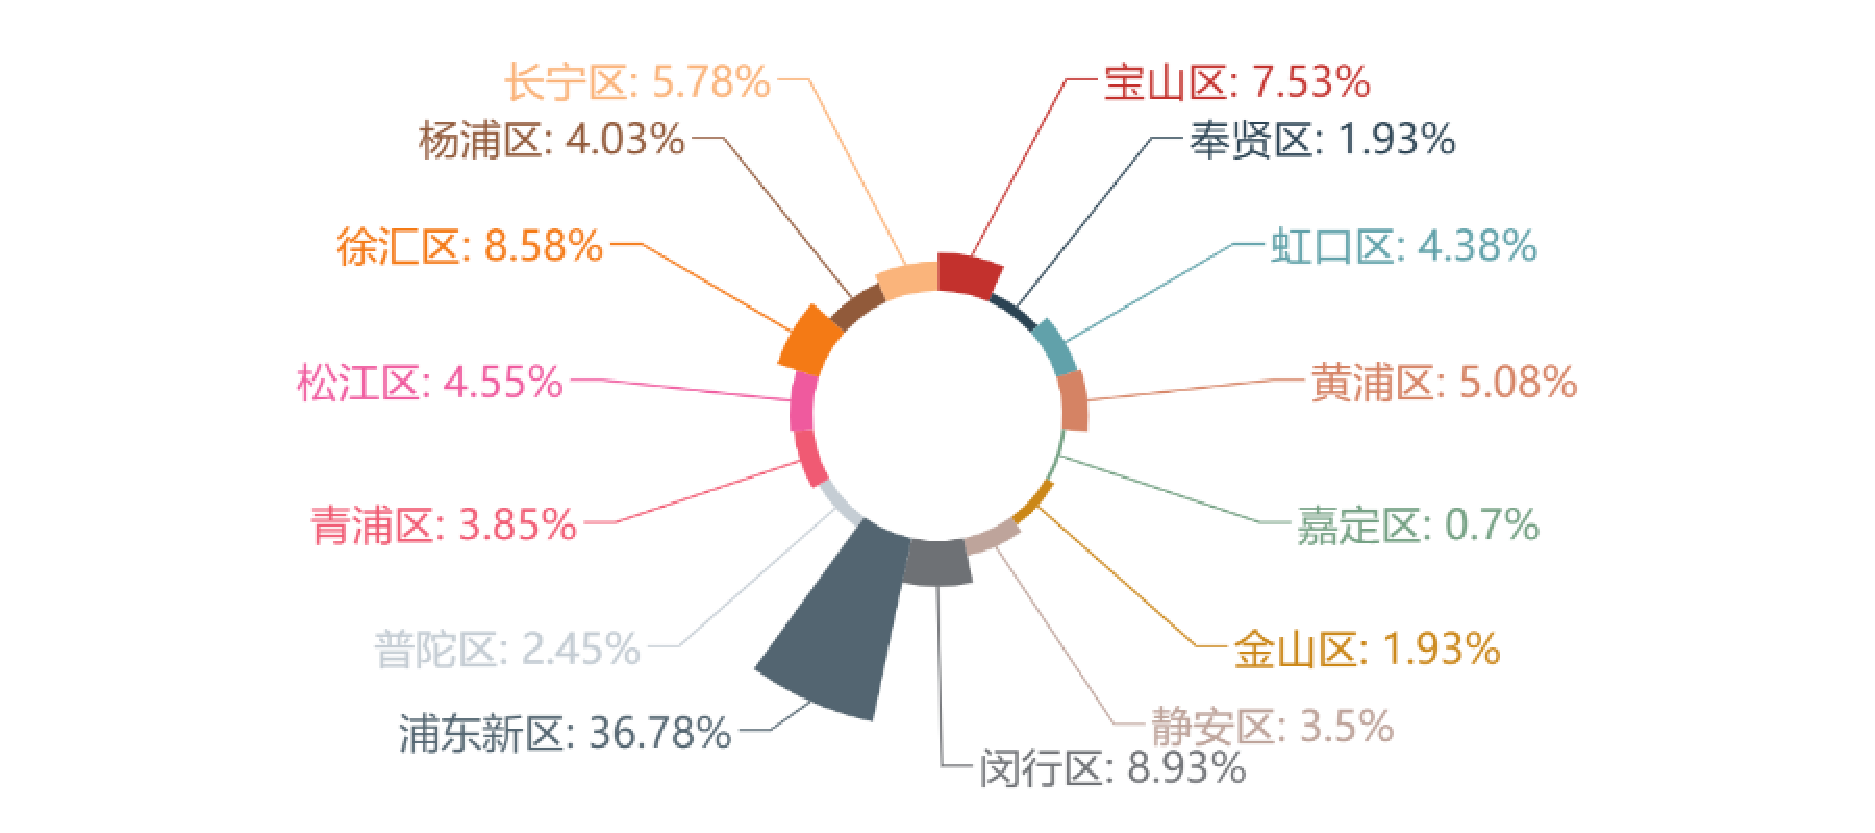
\includegraphics[width=\columnwidth]{./figures/distribution.pdf}
	\centering
	\caption{District Distribution of Charging Stations}
	\label{fig6}
\end{figure}
\subsubsection{Time Frames}
In order to further study stations' use rate in different time periods, we set different time frames, including total time, weekday, weekend, daytime, evening time, morning\_rush hours, evening\_rush hours and travel\_hours, to help observe the use rate discrepancy during these phases. Fig.\ref{fig7} shows the average use-rate of the time frames above.
\begin{figure}[!htp]
	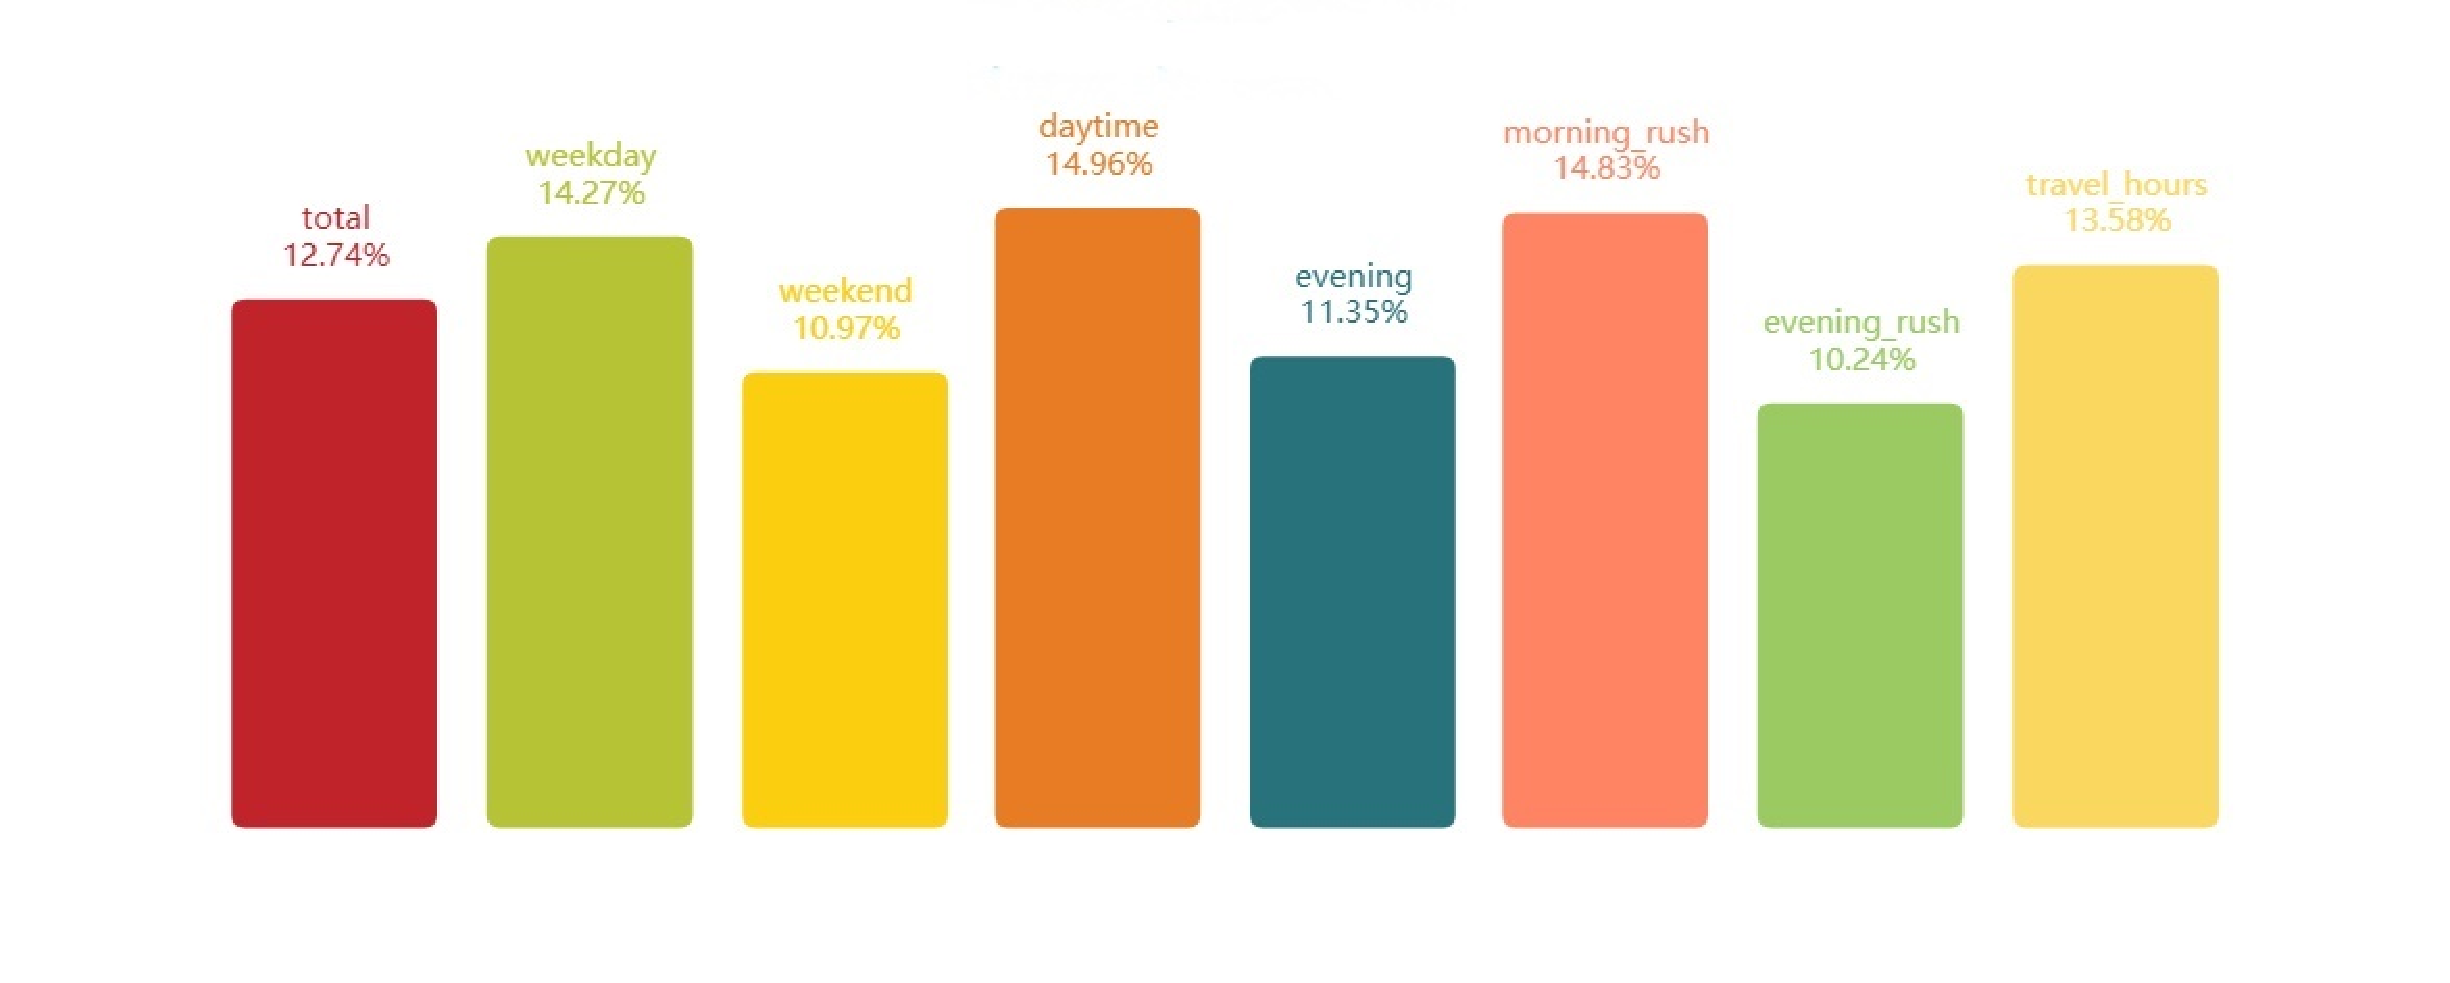
\includegraphics[width=\columnwidth]{./figures/timeframes.pdf}
	\centering
	\caption{Average Use Rate in Different Time Frames}
	\label{fig7}
\end{figure}

\subsection{Preprocessing}
\subsubsection{Data Cleaning}
The original dataset may exist some outliers and missing values, there should be a data cleaning procedure to deal with these invalid data. For outliers, if detected, we remove them from the dataset; for missing values, we use the median filling method to fill blanks with median values computed via 'Imputer' function.

\subsubsection{Feature Zooming}
In 'nearest important POIs', the value of each feature is over hundred, while in other features like 'dc cost fee', the mean value is just about 0.85 per hour. In order to achieve a better performance using machine learning algorithms, we take a feature zooming procedure to normalize feature values so that they can range in [0,1]. Different models may use different zooming strategies, which will be discussed in detail in experiment section. Fig.\ref{fig8} shows an example of the feature 'university' after normalization step.
\begin{figure}[!htp]
	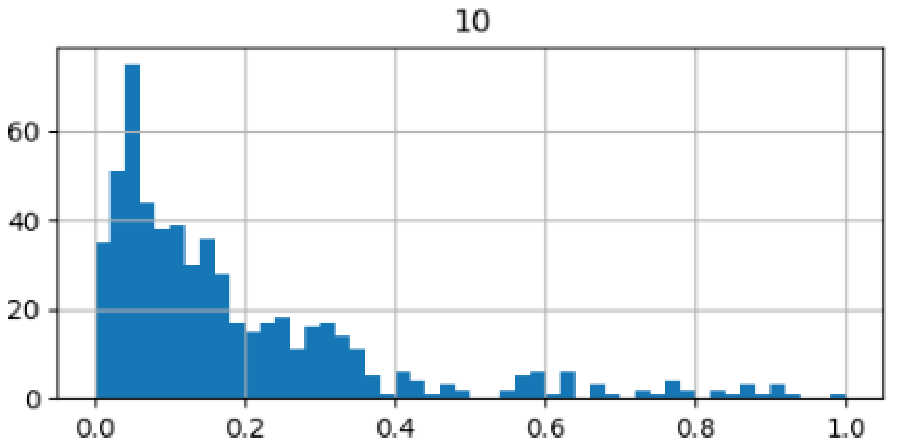
\includegraphics[width=\columnwidth]{./figures/uni.pdf}
	\centering
	\caption{An Example of Feature Normalization}
	\label{fig8}
\end{figure}
\subsection{Implementation}
We aim to implement that when given important features, the model can tell what's the level of a station's use rate. Because the use rate of charging stations range in [0,1), so we set three levels as labels for classification task. In detail, we set use rate from 0 to 20\% as low\_use\_rate; 20\% to 50\% as mid\_use\_rate; and over 50\% as high\_use\_rate. For prediction tasks in both districts dataset and time frames dataset, we take features including stations' surrounding POIs, the number of nearest important POIs(e.g., company, estate, hospital, metro station, shopping center, university), charging port type, charging cost fee and whether it's for private or public use, into consideration. Then we make use of three classification models: SVC, Random Forest and MLP(ANN). With features added into these models, we evaluate the final results and find relationships between classification accuracy and features. The detailed experiment procedure will be discussed in next section.
